% questions.tex —— 1988 年·上海卷 · 题目内容片段（无答案）
% 由 tools/generate_projects.py 依来源总账自 1988/1988_数学真题_上海_试题.md 生成，勿手改（改源 MD 后重跑）


\gkpart{试题}

\begin{gktip}
\textbf{来源说明}：本题面依据固定源 PDF《1988 年全国普通高等学校招生统一考试上海数学试题》逐题转录。固定源共 6 页，题面与“解答及评分标准”排在同一份扫描中：第 1—3 页主要为题面，第 3—6 页含答案与解答。

\textbf{图形说明}：第 2 大题第 8 小题的四个函数图象、第 3 大题第 3 小题的圆锥/圆柱轴截面图和第 5 大题的四面体图依据固定源重绘为 TikZ 矢量图。第 2 大题第 6 小题在固定源扫描中仅见题干；同题名公开 5 页扫描补足了四个选项，现按独立扫描校核录入，来源链接详见 ISSUE-0790。
\end{gktip}

\begin{question}
\gkti{1}

一、（本题满分 30 分）本题共有 10 个小题，只要求直接填写结果。每个空格填对得 3 分，否则一律得零分。

\Needspace{5\baselineskip}
（1） 方程

\nopagebreak[4]
\[
4^x-2^{x+1}-8=0
\]

的解是　　　　。

\Needspace{5\baselineskip}
（2）　

\nopagebreak[4]
\[
y=\sqrt{x-1}
\]

的反函数是　　　　。

（3） 在极坐标系中，以 $\left(\dfrac a2,\dfrac\pi2\right)$ 为圆心、$\dfrac a2$ 为半径的圆的方程为　　　　。

\Needspace{5\baselineskip}
（4） 参数方程

\nopagebreak[4]
\[
\begin{cases}
x=1-2t,\\
y=2t^2-t
\end{cases}
\qquad(t\in\mathbb R)
\]

化为普通方程为　　　　。

（5） 一圆锥的侧面展开图是圆心角为 $216^\circ$ 的扇形，则此圆锥的轴截面的半顶角的正弦是　　　　。

\Needspace{5\baselineskip}
（6）　

\nopagebreak[4]
\[
\lim_{n\to\infty}
\frac{(-2)^{n+1}}{1-2+4-\cdots+(-2)^{n-1}}
\]

的值是　　　　。

\Needspace{5\baselineskip}
（7） 函数

\nopagebreak[4]
\[
y=\cos\left(\frac\pi2x\right)\cos\left[\frac\pi2(x-1)\right]
\]

的最小正周期是　　　　。

（8） 在 $(1+x)^n$ 的展开式中，若第三项和第六项的系数相等，则 $n=$　　　　。

\Needspace{5\baselineskip}
（9） 到椭圆

\nopagebreak[4]
\[
\frac{x^2}{25}+\frac{y^2}{9}=1
\]

右焦点的距离与直线 $x=6$ 的距离相等的动点轨迹方程是　　　　。

（10） 从 6 个运动员中选出 4 人参加 $4\times100$ 米接力赛，如果甲、乙两人都不能跑第一棒，那么共有　　　　种不同的参赛方案（要求结果用数字表示）。

\Needspace{0.4\textheight}
\end{question}
\begin{question}
\gkti{2}

二、（本题满分 30 分）本题共有 10 个小题，每一个小题都给出代号为 A、B、C、D 的四个结论，其中有且只有一个结论是正确的，必须把正确结论的代号写在题后的圆括号内。选对得 3 分，不选、选错或选出的代号超过一个（不论是否都写在圆括号内），一律得零分。

\Needspace{5\baselineskip}
（1） 方程

\nopagebreak[4]
\[
x^4-y^4-4x^2+4y^2=0
\]

所表示的曲线是\mbox{（　　）}

（A）双曲线和一个圆　　（B）两条相交直线

（C）两条平行直线和一个圆　　（D）两条相交直线和一个圆

（2） 在 $\left[-1,\dfrac32\right]$ 上与函数 $y=x$ 相同的函数是\mbox{（　　）}

（A）$y=\arccos(\cos x)$　　（B）$y=\arcsin(\sin x)$

（C）$y=\sin(\arcsin x)$　　（D）$y=\cos(\arccos x)$

\Needspace{5\baselineskip}
（3） 函数

\nopagebreak[4]
\[
y=\frac{1+a^x}{1-a^x}\qquad(a>0,\ a\ne1)
\]

（A）是奇函数　　（B）是偶函数

（C）既是奇函数，又是偶函数　　（D）是非奇非偶函数

（4） $|x|\le2$ 是 $|x+1|<1$ 的\mbox{（　　）}

（A）必要不充分条件　　（B）充分不必要条件

（C）充分必要条件　　（D）既不充分也不必要条件

（5） 下列命题中错误的是\mbox{（　　）}

（A）若一直线垂直于一平面，则此直线必垂直于这平面上所有直线；

（B）若一个平面通过另一个平面的一条垂线，则这两个平面互相垂直；

（C）若一直线垂直于一个平面的一条垂线，则此直线平行于这个平面；

（D）若平面内的一条直线和这个平面的一条斜线的射影垂直，则它也和这条斜线垂直。

（6） 若 $\sin\alpha=\dfrac5{13}$，$\alpha$ 为第二象限角，则 $\operatorname{tg}\dfrac\alpha2$ 的值为\mbox{（　　）}。

（A）$\frac15$　　（B）$5$　　（C）$-5$　　（D）$-\frac15$

\begin{gktip}
\textbf{补证说明}：固定源第 2 页只见题干；上述 A—D 选项由同题名公开 5 页扫描补足，并与固定源第 3 页答案表的 B 相互对应。
\end{gktip}

（7） 在半径为 $a$ 的球中，高为 $\dfrac23a$ 的球冠面积与整个球面面积之和为\mbox{（　　）}

（A）$\frac83\pi a^2$　　（B）$\frac{10}3\pi a^2$　　（C）$\frac{14}3\pi a^2$　　（D）$\frac{16}3\pi a^2$

（8） 下列函数图象中正确的是\mbox{（　　）}
\nopagebreak[4]
\begin{center}% 1988 年上海卷第二大题第 8 小题：四个函数图象选项示意
\begin{tikzpicture}[scale=0.72,>=stealth,font=\scriptsize]
  \begin{scope}[shift={(-3.0,2.25)}]
    \draw[->] (-1.4,0)--(1.65,0) node[right] {$x$};
    \draw[->] (0,-1.1)--(0,1.75) node[above] {$y$};
    \draw[thick] (-1.25,-0.9)--(1.25,1.35);
    \draw[thick,domain=0.08:1.45,samples=60]
      plot (\x,{0.8*ln(\x)/ln(2)});
    \node[above] at (0.7,1.48) {$y=x+a$};
    \node[right] at (1.32,0.35) {$y=\log_2x$};
    \node[below] at (0,-1.45) {（A）};
  \end{scope}
  \begin{scope}[shift={(1.0,2.25)}]
    \draw[->] (-1.4,0)--(1.65,0) node[right] {$x$};
    \draw[->] (0,-1.1)--(0,1.75) node[above] {$y$};
    \draw[thick] (-1.25,-0.9)--(1.25,1.35);
    \draw[thick,domain=-1.25:1.4,samples=80]
      plot (\x,{0.9*exp(-0.85*\x)});
    \node[above right] at (0.35,1.47) {$y=a^x$};
    \node[right] at (1.15,0.45) {$y=x+a$};
    \node[below] at (0,-1.45) {（B）};
  \end{scope}
  \begin{scope}[shift={(-3.0,-1.35)}]
    \draw[->] (-1.4,0)--(1.65,0) node[right] {$x$};
    \draw[->] (0,-1.1)--(0,1.75) node[above] {$y$};
    \draw[thick] (-1.25,-0.9)--(1.25,1.35);
    \draw[thick,domain=0:1.45,samples=70]
      plot (\x,{0.85*\x^0.55});
    \node[above right] at (0.48,1.4) {$y=x^a$};
    \node[below] at (0,-1.45) {（C）};
  \end{scope}
  \begin{scope}[shift={(1.0,-1.35)}]
    \draw[->] (-1.4,0)--(1.65,0) node[right] {$x$};
    \draw[->] (0,-1.1)--(0,1.75) node[above] {$y$};
    \draw[thick] (-1.25,-0.9)--(1.25,1.35);
    \draw[thick,domain=-1.25:-0.08,samples=60]
      plot (\x,{-0.55*sqrt(-\x)});
    \draw[thick,domain=0.08:1.45,samples=60]
      plot (\x,{0.55*sqrt(\x)});
    \node[right] at (0.48,0.73) {$y=x^a$};
    \node[below] at (0,-1.45) {（D）};
  \end{scope}
\end{tikzpicture}
\end{center}
\nopagebreak[4]
（9） 下列关系中正确的是\mbox{（　　）}

（A）$\left(\frac12\right)^{\frac23}<\left(\frac15\right)^{\frac23}<\left(\frac12\right)^{\frac13}$

（B）$\left(\frac12\right)^{-\frac13}<\left(\frac12\right)^{\frac23}<\left(\frac15\right)^{\frac23}$

（C）$\left(\frac15\right)^{-\frac23}<\left(\frac12\right)^{-\frac13}<\left(\frac12\right)^{\frac23}$

（D）$\left(\frac13\right)^{\frac23}<\left(\frac12\right)^{\frac23}<\left(\frac12\right)^{\frac13}$

（10） 方程 $\sin x=\lg x$ 的实数根有\mbox{（　　）}

（A）1 个　　（B）2 个　　（C）3 个　　（D）无穷多个

\Needspace{0.4\textheight}
\end{question}
\begin{question}
\gkti{3}

三、（本题满分 30 分）本题共有 4 个小题，第 1、2 小题等题满分 7 分，第 3、4 小题等题满分 8 分。

\Needspace{5\baselineskip}
（1） 已知直线

\nopagebreak[4]
\[
l_1:3x-y+12=0,\qquad l_2:3x+2y-6=0.
\]

求 $l_1$、$l_2$ 和 $y$ 轴所围成的三角形面积。

\Needspace{5\baselineskip}
（2） 设

\nopagebreak[4]
\[
A=\left\{x\mathrel{}\middle|\mathrel{}x\ge\frac1x,\ x\in\mathbb R\right\},
\qquad
B=\left\{x\mathrel{}\middle|\mathrel{}\sqrt{2x+1}<3,\ x\in\mathbb R\right\}.
\]

求 $D=A\cap B$。

（3） 一个圆锥容器和一个圆柱形容器，它们的轴截面尺寸如图。两容器内盛有的液体的体积正好相等，且液面高度 $h$ 正好相同。求 $h$。
\nopagebreak[4]
\begin{center}% 1988 年上海卷第三题：圆锥、圆柱轴截面示意图
\begin{tikzpicture}[scale=0.7,>=stealth,font=\small]
  \begin{scope}[shift={(-3.0,0)}]
    \coordinate (L) at (-1.55,1.25);
    \coordinate (R) at (1.55,1.25);
    \coordinate (V) at (0,-1.25);
    \draw[thick] (L)--(V)--(R)--cycle;
    \draw[dashed] (0,1.25)--(V);
    \draw[thin] (-1.55,0.25)--(1.55,0.25);
    \draw[<->] (-1.55,1.52)--(0,1.52)
      node[midway,above] {$a$};
    \draw[<->] (-1.85,1.25)--(-1.85,-1.25)
      node[midway,left] {$a$};
    \draw[<->] (1.85,0.25)--(1.85,-1.25)
      node[midway,right] {$h$};
    \node[below] at (0,-1.65) {圆锥};
  \end{scope}
  \begin{scope}[shift={(2.1,0)}]
    \draw[thick] (-1.0,-1.25)--(-1.0,1.25)--(1.0,1.25)--(1.0,-1.25)--cycle;
    \draw[dashed] (0,-1.45)--(0,1.45);
    \draw[thin] (-1.0,0.25)--(1.0,0.25);
    \draw[<->] (-1.0,1.52)--(0,1.52)
      node[midway,above] {$\dfrac a2$};
    \draw[<->] (1.3,0.25)--(1.3,-1.25)
      node[midway,right] {$h$};
    \node[below] at (0,-1.65) {圆柱};
  \end{scope}
\end{tikzpicture}
\end{center}
\nopagebreak[4]
\Needspace{5\baselineskip}
（4） 设方程

\nopagebreak[4]
\[
x^2+3\sqrt3x+4=0
\]

\Needspace{5\baselineskip}
的两个实根为 $x_1\text{、}x_2$。记

\nopagebreak[4]
\[
\alpha=\arctan x_1,\qquad \beta=\arctan x_2.
\]

求 $\alpha+\beta$。

\end{question}
\begin{question}
\gkti{4}

\Needspace{5\baselineskip}
四、（本题满分 15 分）设 $a>0$，$b>0$，

\nopagebreak[4]
\[
y=\log_{\frac12}\left[a^{2x}+2(ab)^x-b^{2x}+1\right].
\]

求使 $y$ 为负值的 $x$ 的取值范围。

\Needspace{0.4\textheight}
\end{question}
\begin{question}
\gkti{5}

五、（本题满分 15 分）本题共有 2 个小题，第 1 小题满分 7 分，第 2 小题满分 8 分。

在棱长都相等的四面体 $A-BCD$ 中，$E\text{、}F$ 分别为棱 $AD\text{、}BC$ 的中点，连接 $AF\text{、}CE$，如图所示。
\nopagebreak[4]
\begin{center}% 1988 年上海卷第五题：正四面体 A-BCD，E/F 为中点
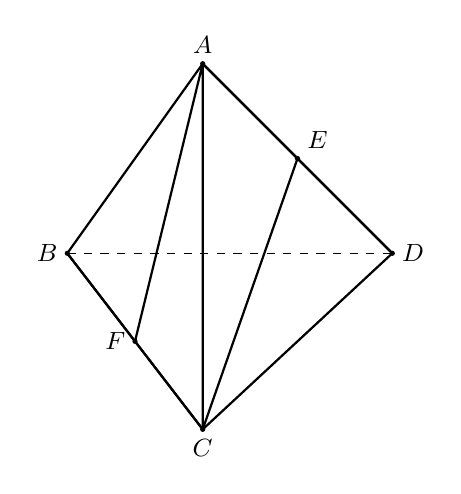
\begin{tikzpicture}[scale=0.86,>=stealth,font=\small]
  \coordinate (A) at (0,3.8);
  \coordinate (B) at (-2.0,1.0);
  \coordinate (C) at (0,-1.6);
  \coordinate (D) at (2.8,1.0);
  \coordinate (E) at (1.4,2.4);
  \coordinate (F) at (-1.0,-0.3);
  \draw[thick] (A)--(B)--(C)--(D)--cycle;
  \draw[thick] (A)--(C) (A)--(F) (C)--(E);
  \draw[dashed] (B)--(D);
  \draw[thick] (B)--(F)--(C);
  \draw[thick] (A)--(E)--(D);
  \fill (A) circle (1.1pt) node[above] {$A$};
  \fill (B) circle (1.1pt) node[left] {$B$};
  \fill (C) circle (1.1pt) node[below] {$C$};
  \fill (D) circle (1.1pt) node[right] {$D$};
  \fill (E) circle (1.1pt) node[above right] {$E$};
  \fill (F) circle (1.1pt) node[left] {$F$};
\end{tikzpicture}
\end{center}
\nopagebreak[4]
（1） 求异面直线 $AF\text{、}CE$ 所成角的大小。

（2） 求 $CE$ 与底面 $BCD$ 所成角的大小（要求角的大小用反三角函数表示）。

\end{question}
\begin{question}
\gkti{6}

\Needspace{5\baselineskip}
六、（本题满分 15 分）复数 $z_1\text{、}z_2\text{、}z_3$ 的辐角分别为 $\alpha\text{、}\beta\text{、}\gamma$，又

\nopagebreak[4]
\[
|z_1|=1,\qquad |z_2|=k,\qquad |z_3|=2-k,
\]

\Needspace{5\baselineskip}
且

\nopagebreak[4]
\[
z_1+z_2+z_3=0.
\]

问 $k$ 各为何值时，$\cos(\beta-\gamma)$ 分别取最大值和最小值，并求出最大值和最小值。

\end{question}
\begin{question}
\gkti{7}

七、（本题满分 15 分）本题共有 2 个小题，第 1 小题满分 5 分，第 2 小题满分 10 分。

\Needspace{5\baselineskip}
在双曲线

\nopagebreak[4]
\[
\frac{y^2}{12}-\frac{x^2}{13}=1
\]

的一支上不同的三点 $A(x_1,y_1)$、$B(\sqrt{26},6)$、$C(x_2,y_2)$ 与焦点 $F(0,5)$ 的距离成等差数列。

（1） 求 $y_1+y_2$。

（2） 证明线段 $AC$ 的垂直平分线经过某一定点，并求该定点的坐标。

\begin{gktip}
题面署名：上海市四平中学　马积祥提供。
\end{gktip}

\end{question}